\documentclass[border=10pt]{standalone}

\usepackage{tikz}
\usetikzlibrary{arrows.meta,arrows,decorations.pathmorphing,backgrounds,positioning,fit,petri,calc,shapes.geometric,scopes,fit,spy}
\usepackage{pgfplots}
\pgfplotsset{,compat=1.11}
\tikzset{/pgf/number format/1000 sep={\,}}

\usepackage{fontawesome5}
\renewcommand{\familydefault}{\sfdefault}
\usepackage{helvet}
\begin{document}

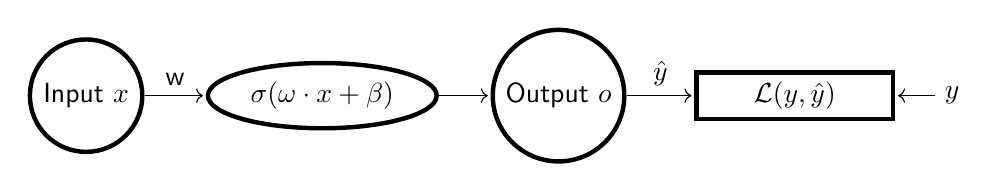
\begin{tikzpicture}[shorten >=1pt,node distance=3cm,auto]
   
   \node[ultra thick, draw, circle] (input) {Input $x$};
   \node[ultra thick, draw, ellipse] (hidden) [right of=input] {$\sigma(\omega \cdot x + \beta)$};
   \node[ultra thick, draw, circle] (output) [right of=hidden] {Output $o$};
   \node[ultra thick, draw, rectangle, minimum width=2.5cm] (loss) [right of=output] {$\mathcal{L}(y, \hat{y})$};

   \path[->] (input) edge node {w} (hidden)
   (hidden) edge (output)
   (output) edge node {$\hat{y}$} (loss);

   \node (ytrue) [right of=loss, node distance=2cm] {$y$};
   \path[->] (ytrue) edge (loss);
   
 \end{tikzpicture}
\end{document}
